\documentclass[a4paper, 12pt]{article}

\usepackage[T1]{fontenc}
\usepackage[utf8]{inputenc}
\usepackage{lmodern}
\usepackage[bottom]{footmisc}

\setlength{\parindent}{0pt}
\setlength{\parskip}{0.8em}

\usepackage{geometry}
\geometry{margin=1in}

\usepackage{amsmath,amssymb,mathtools}
\usepackage{pgfplots}
\pgfplotsset{compat=1.18}
\usepackage{tikz}
\usepackage[justification=centering]{caption}
\usepackage{float}    % for [H] placement
\usepackage{placeins} % for \FloatBarrier
\usepackage{hyperref}
\hypersetup{
    colorlinks=true,
    linkcolor=black,
    urlcolor=blue
}

% Packages and styling from the distribution code
\usepackage{titlesec}
\titlespacing*{\section}{0pt}{2ex}{1ex}
\titlespacing*{\subsection}{0pt}{1.5ex}{0.5ex}
\usepackage{graphicx} 
\usepackage{blindtext}
\usepackage{setspace} % Includes \doublespacing
\usepackage{lastpage}
\usepackage{comment}
\usepackage{fancyhdr}
\usepackage{enumitem}
\usepackage{natbib}
\usepackage{url}
\usepackage{ulem}
\usepackage{multirow}

% Counters from the distribution code
\counterwithin{figure}{section}
\counterwithin{equation}{section}

\begin{document}

\doublespacing % Apply double spacing

\begin{titlepage}
    \begin{center}
    
        \vspace*{2cm}
        {\Huge \textbf{A Comparative Approach to Taylor Polynomials and Padé Approximants}\par}
        
        \vspace{1.5cm}
        {\Large \textbf{Pingan Yao}\par} % Author's name
        
        \vspace{2cm}
        \Large
        \textbf{Research Question:}
        
        \vspace{0.5cm}
        \LARGE To what extent do Padé Approximants offer a superior approximation to Taylor Polynomials for transcendental functions near singularities or outside the radius of convergence?

        \vspace{1.5cm}

        \Large
        October 2025, Mathematics\\
        Word Count:
        
    \end{center}
\end{titlepage}

\newpage

\pagenumbering{roman}
\tableofcontents
\newpage
\listoffigures

\newpage

\pagenumbering{arabic}
\setcounter{page}{1}

\section{Introduction} 
% Placeholder for Introduction section, as required by the standard structure.

\section{Mathematical background} % This will be Section 2

\subsection{Approximation of functions}
Function approximation refers to the process of estimating a complex function with a simpler one that closely matches the original, often within a certain region. Approximating functions is an integral tool in the field of calculus and real analysis, as many functions cannot be expressed using elementary, algebraic operations, making it extremely difficult to calculate and analyse their behaviour, a task which is essential when using functions to predict a model or bahaviour in all mathematics-related fields. Function approximation provides a powerful method to simplify such complex functions into something that is highly similar to the original function, while also being easy to analyse and fast to compute. This is the case due to the fact that the simpler functions are often expressed as a polynomial, a rational function, trigonometric sum, etc., which can be much more easily differentiated in comparison to the complex functions. It allows mathematicians to more efficiently estimate function values numerically, simplify integrals or differential equations, and understand the local behaviour of functions. The branch of mathematical analysis concerned with how functions can best be approximated with simpler functions is known as approximation theory. In reality, there are many different methods to approximate functions, each with their own advantages and disadvantages. Depending on the original function and use case, it is important to determine the most suitable approximation method to achieve the best possible result. 

\subsection{Taylor Polynomials}
One of the most widely-used, fundamental methods of function approximation is through the Taylor polynomials. It is an approximation of an $n$-times differentiable function around a given point by a polynomial of degree $n$. 

Suppose a continuous function $f$ that is $n$-times differentiable at some point $a$. The Taylor polynomial of degree $n$ centred at $a$, as defined by Taylor’s theorem, is as follows:
\begin{equation}
T_n(x) = f(a) + f'(a)(x-a) + \frac{f''(a)}{2!}(x-a)^2 + \frac{f^{(3)}(a)}{3!}(x-a)^3 + \cdots + \frac{f^{(n)}(a)}{n!}(x-a)^n,
\end{equation}
or more simply using summation notation:
\begin{equation}
T_n(x) = \sum_{k=0}^{n} \frac{f^{(k)}(a)}{k!}(x-a)^k .
\end{equation}

This often allows a highly accurate local approximation of the function around $a$, as the polynomial takes into account the derivative information of $f$, allowing it to mimic similar local behaviour, where specifically:
\begin{itemize}
    \item the term $f(a)$ allows it to have the same value at $a$ as $f$
    \item $f'(a)$ dictates the slope of the function at $a$, matching the polynomial’s tangent line to that of $f$
    \item $f''(a)$ dictates the curvature at $a$
    \item higher-order derivatives provide further information about $f$’s rates of change, allowing more exact approximations.
\end{itemize}

Thus, the more terms the Taylor polynomial includes, the closer the polynomial resembles the actual function. In practice, if $f$ is infinitely differentiable at $a$, an infinite sum of terms calculated from the function’s derivatives can be written as:
\begin{equation}
f(x)=\sum_{n=0}^{\infty} \frac{f^{(n)}(a)}{n!}(x-a)^n .
\end{equation}
This is known as a Taylor series. In daily applications, however, it often suffices to approximate a function with a Taylor polynomial of the $n$th degree, at the cost of less accurate approximations, but for the benefit of reduced computational demand.

As an example, we compute a Taylor polynomial of the function $f(x)=\cos x$ where $a=0$:
\begin{enumerate}
\item $\cos 0 = 1$, so the first term of the polynomial, $f(a)=1$;
\item The derivative of $\cos x$, $f'(x) = - \sin x$. Therefore, the slope of $f$ at $x=0$ is equal to $0$. This means that for the best approximation, the polynomial should have a tangent line of slope $0$ at $x=0$. Plugging into the equation, the second term becomes $\dfrac{f'(0)}{1!}(x-0)^1 = 0$, which is simply $0$. The second term of the polynomial, therefore, is $0$. Plotting the current polynomial alongside the graph of $f$ gives its tangent line at $x=0$ (figure~\ref{fig:t1});
\end{enumerate}

\begin{figure}[H]
\centering
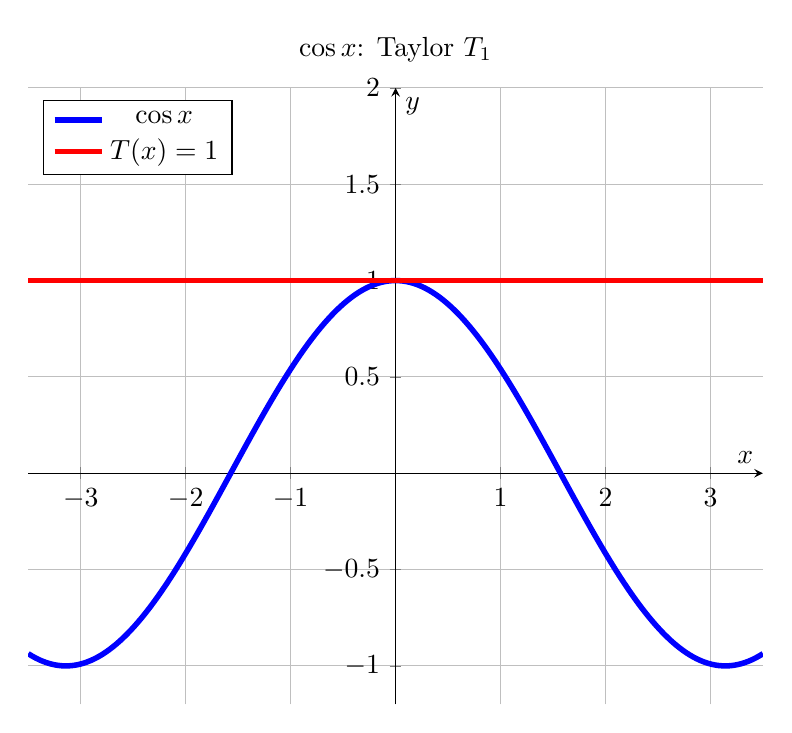
\begin{tikzpicture}
\begin{axis}[
    axis lines=middle,
    width=0.9\linewidth,
    xlabel={$x$}, ylabel={$y$},
    title={$\cos x$: Taylor $T_1$},
    grid=both, legend style={at={(0.02,0.98)},anchor=north west},
    domain=-3.5:3.5, samples=201,
    ymin=-1.2, ymax=2,
]
    \addplot[color=blue, line width=2pt] {cos(deg(x))};
    \addlegendentry{$\cos x$}
    \addplot[color=red, line width=2pt] {1};
    \addlegendentry{$T(x)=1$}
\end{axis}
\end{tikzpicture}
\caption{Tangent of $\cos x$ about $x=0$ with the 1st-degree Taylor polynomial.}
\label{fig:t1}
\end{figure}

\begin{enumerate}
\setcounter{enumi}{2}
\item The second derivative of $f$, $f''(x) = - \cos x$. Therefore, the curvature of $f$ at $x=0$ is equal to $-1$. Similarly, this should be the case for our Taylor polynomial. Plugging into the equation, the third term of the polynomial can be expressed $\dfrac{f''(0)}{2!}(x-0)^2$, which can be simplified as $-\frac{1}{2}x^2$.
\end{enumerate}
This gives us the Taylor polynomial of the 2nd degree for $f$: 
\begin{equation}
T_2(x) = 1 - \frac{1}{2}x^2 .
\end{equation}
When plotted alongside $f$, we see the approximation in figure~\ref{fig:t2}. As can be seen, the polynomial gives a rather accurate approximation for small values of $|x|$.

\begin{figure}[H]
\centering
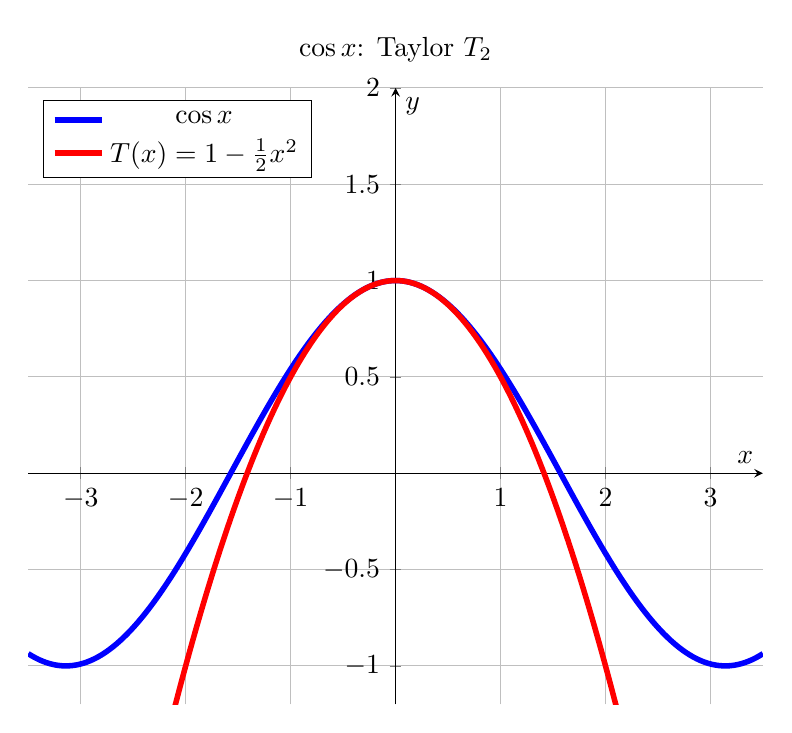
\begin{tikzpicture}
\begin{axis}[
    axis lines=middle,
    width=0.9\linewidth,
    xlabel={$x$}, ylabel={$y$},
    title={$\cos x$: Taylor $T_2$},
    grid=both, legend style={at={(0.02,0.98)},anchor=north west},
    domain=-3.5:3.5, samples=201,
    ymin=-1.2, ymax=2,
]
    \addplot[color=blue, line width=2pt] {cos(deg(x))};
    \addlegendentry{$\cos x$}
    \addplot[color=red, line width=2pt] {1-(1/2)*x^2};
    \addlegendentry{$T(x)=1-{1\over2}x^2$}
\end{axis}
\end{tikzpicture}
\caption{Approximation of $\cos x$ about $x=0$ with the 2nd-degree Taylor polynomial.}
\label{fig:t2}
\end{figure}

More terms of higher power can be computed to give more accurate approximations of the function. The fourth term of the Taylor polynomial of $f$ is 0, and the fifth term is $\dfrac{1}{24}x^4$. Thus, the 4th degree Taylor polynomial is 
\begin{equation}
T_4(x) = 1 - \frac{1}{2}x^2 + \frac{1}{24}x^4 .
\end{equation}
Plotting this gives a highly accurate approximation of $f$, as shown in figure~\ref{fig:t4}. In Section 4, a systematic method of calculating accuracy of the approximation will be presented.

\begin{figure}[H]
\centering
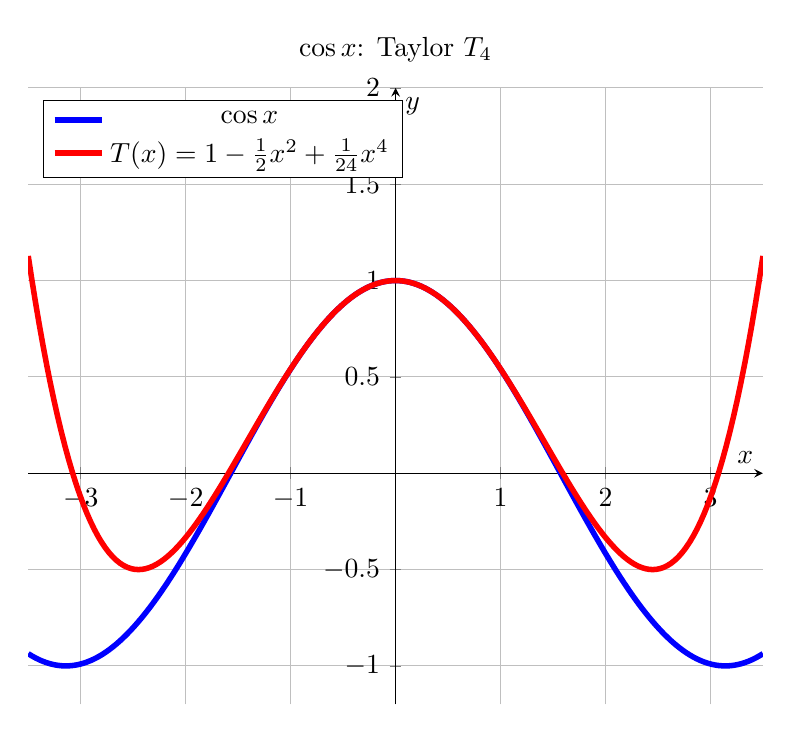
\begin{tikzpicture}
\begin{axis}[
    axis lines=middle,
    width=0.9\linewidth,
    xlabel={$x$}, ylabel={$y$},
    title={$\cos x$: Taylor $T_4$},
    grid=both, legend style={at={(0.02,0.98)},anchor=north west},
    domain=-3.5:3.5, samples=201,
    ymin=-1.2, ymax=2,
]
    \addplot[color=blue, line width=2pt] {cos(deg(x))};
    \addlegendentry{$\cos x$}
    \addplot[color=red, line width=2pt] {1-(1/2)*x^2+(1/24)*x^4};
    \addlegendentry{$T(x)=1-{1\over2}x^2+{1\over24}x^4$}
\end{axis}
\end{tikzpicture}
\caption{Approximation of $\cos x$ about $x=0$ with the 4th-degree Taylor polynomial.}
\label{fig:t4}
\end{figure}

The special case of a Taylor series centred at $a=0$ is known as a Maclaurin series. The polynomial we just computed above consistutes the first few terms of the Maclaurin series for $f$. The Maclaurin series can be written as:
\begin{equation}
f(x)=\sum_{n=0}^{\infty} \frac{f^{(n)}(0)}{n!}x^n .
\end{equation}

\FloatBarrier

\subsection{Padé Approximants}
There exists a “best” approximation of a function near a specific point by a rational function. This is known as a Padé approximant, which approximates a function as a ratio of two polynomials. An $[N/M]$ Padé approximant is formed of an $M$th degree polynomial on the numerator and an $N$th degree polynomial on the denominator. This can be expressed as:
\begin{equation}
R^N_M(x)=\frac{a_0 + a_1x + a_2x^2 + \cdots + a_M x^M}{1 + b_1x + b_2x^2 + \cdots + b_N x^N}=\frac{\sum_{j=0}^{M} a_j x^j}{1+\sum_{k=1}^{N} b_k x^k}.\;\;\;
\footnote{In principle, the constant “1” in the denominator should be $b_0$. To simplify algebraic processes, we let $b_0=1$ without loss of generality.}\end{equation}

The Padé approximant $R^N_M$ to a function $f(x)$ is defined such that its Maclaurin series expansion matches the Maclaurin series of $f$ up to the highest possible order. This means that:
\begin{equation}
f(0)=R(0),\quad f'(0)=R'(0),\quad f''(0)=R''(0),\ \ldots,\ f^{(M+N)}(0)=R^{(M+N)}(0).
\end{equation}
Formally,
\begin{equation}
f(x) - R^N_M(x) = \mathcal{O}(x^{M+N+1}) \quad \text{as } x \to 0.
\end{equation}
Therefore, to compute the $[N/M]$ Padé approximant of a function $f(x)$, we need to equate it to the function’s Taylor series at $a=0$ up to order $M+N$.

As an example, the process of constructing a $[2/2]$ Padé approximation of $\cos x$ is as follows.
We equate the $[2/2]$ Padé approximant with the unknown coefficients, to the 4th degree Taylor polynomial of $\cos x$, $T_4(x) = 1 - \frac12 x^2 + \frac{1}{24}x^4$, which we previously computed:
\begin{equation}
\frac{a_0 + a_1x + a_2x^2}{1 + b_1x + b_2x^2}
= 1 - \frac{x^2}{2} + \frac{x^4}{24} + \mathcal{O}(x^5).\;\;\;
\footnote{The notation $\mathcal{O}(x^5)$ indicates that $\cos x$ and its [2/2] Padé approximant match up to the $x^4$ term, and their difference only begins at terms of order $x^5$ or higher.}\end{equation}
Multiplying both sides by the denominator of the Padé approximant,
\begin{equation}
a_0 + a_1x + a_2x^2 = (1 + b_1x + b_2x^2)\!\left(1 - \frac{x^2}{2} + \frac{x^4}{24}\right).
\end{equation}
Expanding the right hand side:
\begin{equation}
a_0 + a_1x + a_2x^2 = 1 + b_1x + \left(b_2-\frac12\right)x^2 - \frac{b_1}{2}x^3 + \left(\frac{1}{24}-\frac{b_2}{2}\right)x^4 + \cdots
\end{equation}
We are only computing $[2/2]$, we can discard any term on the RHS that has power of $x$ higher than $4$.
To solve for the unknown values, we equate the coefficients of the terms for each power of $x$ on both sides:
\begin{align}
a_0 &= 1, & a_1 &= b_1, & a_2 &= b_2 - \frac12, & 0 &= -\frac{b_1}{2}, & 0 &= \frac{1}{24} - \frac{b_2}{2} .
\end{align}
$b_1$ and $b_2$ can be easily solved from equations where $b_1 = 0$ and $b_2 = \frac{1}{12}$. Plugging these into the second and third equations yields $a_1 = 0$, and $a_2 = -\frac{5}{12}$.
Having all coefficients solved, we can then write the $[2/2]$ Padé approximant of $\cos x$:
\begin{equation}
R^2_2(x) = \frac{1 - \frac{5}{12}x^2}{1 + \frac{1}{12}x^2}.
\end{equation}

\begin{figure}[H]
\centering
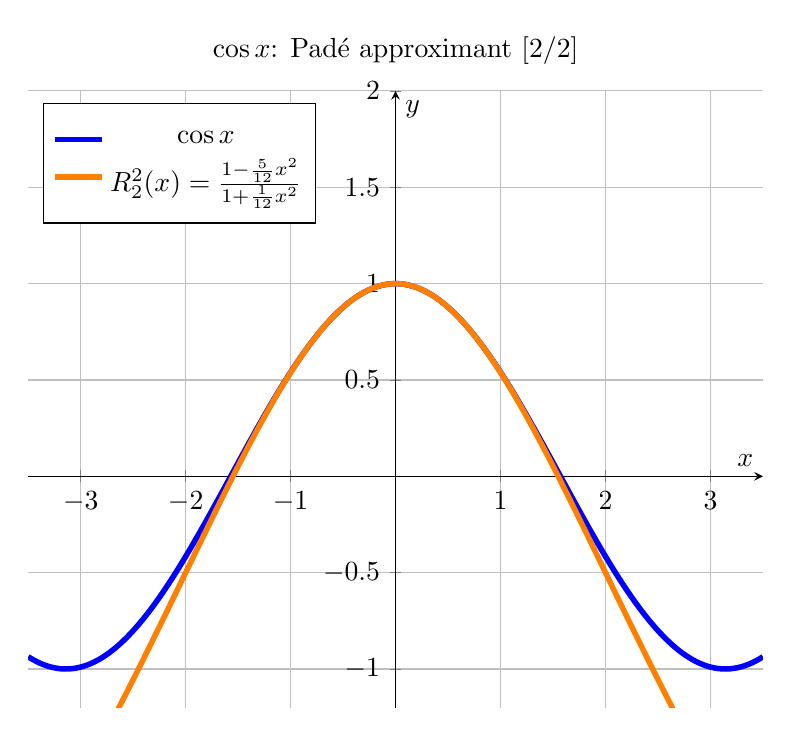
\begin{tikzpicture}
\begin{axis}[
axis lines=middle,
    width=0.9\linewidth,
    xlabel={$x$}, ylabel={$y$},
    title={$\cos x$: Padé approximant $[2/2]$},
    grid=both, legend style={at={(0.02,0.98)},anchor=north west,inner ysep=8pt},
    domain=-3.5:3.5, samples=201,
    ymin=-1.2, ymax=2,
]
    \addplot[color=blue, line width=2pt] {cos(deg(x))};
    \addlegendentry{$\cos x$}
    \addplot[color=orange, line width=2pt] {(1-(5/12)*x^2)/(1+(1/12)*x^2)};
    \addlegendentry{$R^2_2(x)={{1-{5\over12}x^2}\over{1+{1\over12}x^2}}$}
\end{axis}
\end{tikzpicture}
\caption{Approximation of $\cos x$ with the [2/2] Padé approximant.}
\label{fig:pade22}
\end{figure}

\FloatBarrier

\subsection{Transcendental Functions}
A transcendental function is defined as a function that cannot be obtained by a finite number of operations as a solution of an algebraic equation. Transcendental functions cannot be expressed only by algebraic operations (addition, subtraction, multiplication, and division), and must be written with advanced operations.

Common examples of transcendental functions include exponential functions (e.g. $e^x$), logarithmic functions (e.g. $\ln x, \log x$), and trigonometric functions (e.g. $\sin x, \cos x, \tan x$).

This research will focus specifically on transcendental functions, as their characteristics often make approximation by Taylor polynomials problematic (see \textbf{Section 2.5}).

\subsection{Limitations of Taylor Approximation} 
When approximating functions, it is useful for the approximation to represent as much information about the original function as possible. This not only includes the values of $f(x)$ across a wide range of $x$ values, but also certain behaviours of a function due to points known as singularities. The Taylor series are often limited by its radius of convergence, as well as its lack of ability to reflect singularities, where points in the original function are undefined.

\subsubsection{Convergence}
In the context of function approximation using series, convergence is the property of a function to approach a finite value (known as the limit) more and more  closely as its number of terms increases. A series is said to converge if the sum gets closer to a specific finite value as we keep adding more terms. Formally, a series $\sum a_n$ converges if:

\begin{equation}
\lim_{N \to \infty} S_N = \lim_{N \to \infty} \sum_{n=0}^{N} a_n \;\text{exists}.
\end{equation}

Otherwise, the series diverges. 

For a Taylor series, we are interested in whether the approximation converges at some value of $x$. The series might converge for some values of $x$, but not for others. A Taylor polynomial of degree $N$ is known as a partial sum $S_N(x)$ of the series. A Taylor series converges when the sequence of partial sums has a limit as $N\to\infty$:

\begin{equation}
    \lim_{N\to\infty} S_N(x)=L(x)
\end{equation}
where $L(x)$ is the limit.

If the limit $L(x)$ is equal to the original function $f(x)$, the Taylor series is said to converge to the function at that $x$. This means that as the number of terms of the Taylor polynomial increases, it approaches the original function, making the approximation useful for analysis. 

When a Taylor series is computed around a point $a$, there is always a region around $a$ where the series converges. However, the Taylor approximation often fails to converge for all $x$. Beyond the said region, the Taylor series can diverge, failing to sum to a finite value and approximate $f(x)$.

The region where a Taylor series converges is symmetric across $a$, and its size is known as the radius of convergence, which can be denoted by $R$.
\begin{equation}
\begin{aligned}
\text{If } |x - a| < R &\Rightarrow \text{ the series converges},\\
\text{If } |x - a| > R &\Rightarrow \text{ the series diverges.}
\end{aligned}
\end{equation}

The radius of convergence for a Taylor series can be found by using the ratio test, where, given a series $\sum c_n(x-a)^n$:
\begin{equation}
    \lim_{n\to\infty}\left| {c_{n+1}\over{c_n}}\right|=L
\end{equation}
Where:
\begin{equation}
    R={1\over L}
\end{equation}
\begin{itemize}
    \item If $L=0,\;R=\infty$, so the Taylor series converges everywhere;
    \item If $L=\infty,\; R=0$, so the Taylor series only converges at $x=a$.
\end{itemize}

Outside the radius of convergence, the Taylor series fails to be analytical. It stops following the behaviour of the original function, making it ineffectual in analysis. 

An example of a function where the Taylor series fails to approximate for a large interval of $x$ is $f(x)=\ln(1+x)$, whose Taylor series is given by $\sum_{n=1}^{\infty}(-1)^{n+1}{x^n\over n}$. Using the ratio test, we find that its radius of convergence is 1. Thus, the series only converges for $|x|<1$. Plotting the 10th-degree Taylor polynomial alongside the original function yields the following graph.

\begin{figure}[H]
\centering
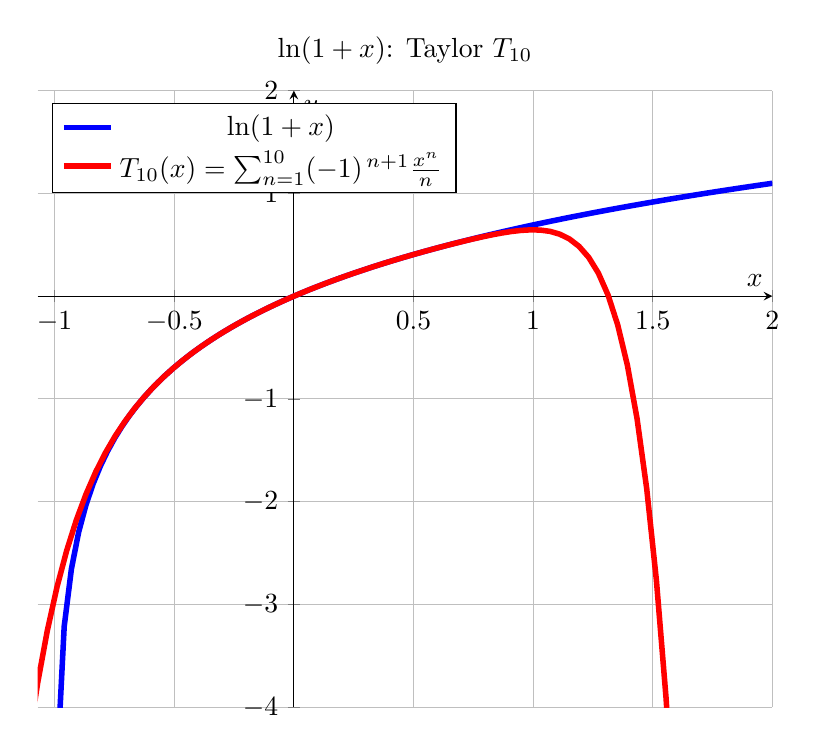
\begin{tikzpicture}
\begin{axis}[
    axis lines=middle,
    width=0.9\linewidth,
    xlabel={$x$}, ylabel={$y$},
    title={$\ln(1+x)$: Taylor $T_{10}$},
    grid=both,
    legend style={at={(0.02,0.98)},anchor=north west},
    ymin=-4, ymax=2,
    domain=-2:2, samples=100,
]
    % log curve: skip x \le -1 to avoid the blow-up
    \addplot[color=blue, line width=2pt, domain=-0.99:2, unbounded coords=jump]
        {ln(1+x)};
    \addlegendentry{$\ln(1+x)$}

    % 10th-degree Taylor polynomial
    \addplot[color=red, line width=2pt, domain=-2:2]
        {x - x^2/2 + x^3/3 - x^4/4 + x^5/5
         - x^6/6 + x^7/7 - x^8/8 + x^9/9 - x^10/10};
    \addlegendentry{$T_{10}(x)=\sum_{n=1}^{10}(-1)^{\,n+1}\frac{x^{n}}{n}$}
\end{axis}
\end{tikzpicture}
\caption{Approximation of $\ln(1+x)$ with the 10th-degree Taylor polynomial}
\end{figure}

As can be seen, between -1 and 1, the Taylor polynomial offers a good approximation of $f(x)$. However, outside this interval, the polynomial immediately diverges. The approximation outside the radius of convergence does not improve even if more terms are added to the polynomial. For this function specifically, anything beyond the interval of $-1<x<1$ cannot be analysed with Taylor approximation.

As it turns out, this happens to be the case for many functions when being approximated by a Taylor polynomial. It is one of its major limitations, where, oftentimes its terms do not offer a method of approximating larger intervals.

\subsubsection{Singularities}
A function is defined to be analytic at a point $a$ if the function can be written exactly as a convergent Taylor series around that point. Otherwise, the point is known as a singularity, at which the function ceases to be analytic.

Singularities among transcendental functions are mostly concerned with points that are undefined. Taylor polynomials usually fail to model the behaviour of a function at these points.

\underline{\textbf{Pole}}

The most common type of singularity where Taylor approximation struggles is pole. A pole is a point where a function approaches positive or negative infinity, commonly shown as vertical asymptotes. Taylor polynomials fail at poles because they are built on the assumption that the function is smooth and continuous. Poles, which effectively breaks a function on its two sides, are not reflected in the derivative information used in the Taylor polynomial calculations. As an example, the 10th-degree Maclaurin polynomial of the transcendental function $f(x)=\frac{e^x}{x+1}$ are plotted as follows. 

\begin{figure}[H]
\centering
\begin{tikzpicture}
\begin{axis}[
    axis lines=middle,
    width=0.9\linewidth,
    xlabel={$x$}, ylabel={$y$},
    title={$\frac{e^x}{x+1}$: Taylor $T_{10}$},
    grid=both,
    legend style={at={(0.02,0.98)},anchor=north west, row sep=7pt},
    ymin=-2, ymax=6,
    domain=-2:2, samples=120,
]

    % Actual function (skip the pole at x = -1)
    \addplot[color=blue, line width=2pt, unbounded coords=jump]
        {exp(x)/(x+1)};
    \addlegendentry{$\dfrac{e^x}{x+1}$}

    % 10th-degree Maclaurin polynomial
    \addplot[color=red, line width=2pt]
        {1
        + 0*x
        + (1/2)*x^2
        - (1/3)*x^3
        + (3/8)*x^4
        - (11/30)*x^5
        + (53/144)*x^6
        - (103/280)*x^7
        + (14833/40320)*x^8
        - (16687/45360)*x^9
        + (1334961/3628800)*x^10};
    \addlegendentry{$T_{10}(x)$}

    \addplot[dashed, black, line width=1pt, forget plot] coordinates {(-1,-2) (-1,6)};


\end{axis}
\end{tikzpicture}
\caption{Approximation of $\dfrac{e^x}{x+1}$ with the 10th-degree Taylor polynomial}
\end{figure}

As can be seen, due to the rational structure of the function, -1 is a pole, and thus the approximation diverges from the original function as it approaches the pole. The series, as a result, has a radius of convergence of 1.

\underline{\textbf{Branch Point}}

Branch point is a type of singularity used to describe when a function becomes multi-valued, such as in the case of $f(x)=\ln (1+x)$ at $x=-1$. As already seen in \textbf{Section 2.5.1}, Taylor approximation fails at such singularities, as polynomials cannot represent branching.

\underline{\textbf{Removable Singularity}}

For the special case of removable singularities, there exists a finite limit. As a result, even though the point is undefined, the function is analytic at that point, as the limit can be removed.

The classic example of removable singularity is $f(x)=\frac{\sin x}{x}$ at $x=0$. The function remains continuous despite the singularity. Thus, in this case, Taylor polynomials remain effective.

As can be noticed in the above examples, the closest singularity of a function to the expansion point of a Taylor series dictates its radius of convergence.

\section{Research Objective} 
In this research, we aim to develop a systematic method to compare transcendental function approximations using Taylor polynomials and Padé approximants. Using this method, we will determine if, and to what extent, Padé approximant is superior to Taylor polynomials in the aforementioned scenarios where Taylor fails to be effective. We will then explore the mathematical reasons behind the comparison outcome.

In the context of this research, we define superiority in function approximation of comparable orders as follows:

\begin{itemize}
  \item The approximation follows the original function with smaller maximum error over a specified domain outside the radius of convergence.
  \item The approximation more accurately models the structural behaviour of the original function near singularities, particularly by producing divergence or asymptotic features.
\end{itemize}

\section{Methodology} 

The research will study four specific transcendental functions for comparison between Taylor polynomials and Padé approximants. The functions are:

\begin{itemize}
  \item $f(x)=\tan x$
  \item $f(x)=\arctan x$
  \item $f(x)=\ln (1+x)$
  \item $f(x)=\frac{e^x}{1+x}$
\end{itemize}

These functions are selected to cover the most common types of transcendental functions, as aforementioned. Collectively, they include the key features relevant to this investigation, including vertical and horizontal asymptotes, as well as other singularities.

For each function, we will calculate the 6th-degree and 10th-degree Taylor polynomials with 0 as the expansion point. Using the polynomials, we will compute the [3/3] and [5/5] Padé approximants, which match the respective Taylor approximations. Two different orders will be used in the investigation, so that any accuracy variations with increasing order can be observed, improving the reliability of the results.

We will then test three regions of the function, for both orders.

\subsection{Inside Radius of Convergence}
This will serve as a baseline for our investigation. Within the radius of convergence, Taylor series is theoretically guaranteed to converge to the function. Therefore, this will be a control region, allowing us to establish performance of the two approximation methods in a well-behaved domain. 

The region inside the Taylor radius of a function will be denoted $I_1$ henceforth. In addition, we define our tested region to be:

\begin{equation*}
I_1: |x| < 0.8R
\end{equation*}

The domain is reduced from the full radius of convergence as Taylor polynomials tend to lose accuracy as the $x$ value approaches the boundary, since singularity exerts analytic influence. 

To compare the two approximation methods, we will compute the \textbf{maximum absolute error (MAE)} for Taylor and Padé compared to the original function within the region, where MAE can be defined as:

\begin{equation}
    E_{\max}(I)=\max_{x\in I}\left|f(x)-A(x)\right|
\end{equation}

Where:

\begin{itemize}
    \item $f(x)$ is the original function,
    \item $A(x)$ is the approximation (Taylor / Padé)
\end{itemize}

Due to maximum absolute error involving a supremum over a continuum of points, it is generally not feasible to evaluate these functions analytically. Thus, we will compute this value through numerical evaluation.

Using a custom Python program, the maximum absolute error can be estimated using a dense uniform grid, by computing the function values at regularly spaced points across the interval. For our investigation, we will sample points with a step size of $h = 0.001$, which will produce close estimations of the error, given that the functions being studied are smooth.\footnote{The Python program used for this research, as well as the resulting datasets, are archived in GitHub, available through the link in the appendix.}

We will then compare the results for Taylor polynomial and Padé approximant. 

\subsection{Outside Radius of Convergence}
This region is our main domain of interest. Established by the aforementioned theory, we expect to see a larger discrepancy between the two approximation methods here. We denote the region outside the Taylor radius of a function $I_2$, where:

\begin{equation*}
    I_2: 1.2R < |x| < 2R
\end{equation*}

Similarly as before, this domain allows us to exclude the points immediately surrounding the radius of convergence, avoiding unbounded errors that do not reflect the performance of the approximations.

We will follow the same procedure to that described in \textbf{Section 4.1} to compute the MAE for $I_2$ numerically. However, as $I_2$ can comprise two regions for each function (one outside each boundary), we will only test one region, which is sufficient for our comparison.

For consistency, we will use the right side $I_2$ for all four functions. For $f(x)=\tan (x)$ and $f(x)=\arctan x$, whose singularities are symmetric across the expansion point, we expect identical results regardless of the side tested. For $f(x)=\ln(1+x)$ and $f(x)=\frac{e^x}{1+x}$, whose radius is bounded by singularity on one side, the right side will be the opposite side where the original function remains defined.

\subsection{Near Singularities}
We are interested in whether Padé approximants can consistently capture singular behaviour, which Taylor fails at. Also key to our investigation is to explore the extent to which Padé approximants are reliable in the region near singularities, which we denote $I_3$. We will focus solely on the region within the radius of convergence approaching the singularity, where all four functions are well defined. We define $I_3$ as:

\begin{equation*}
    I_3= 0.9R < |x| < (R-\delta)
\end{equation*}

Where $\delta = 10^{-6}R$. This is a buffer that excludes the singularity point from the region, which would otherwise be undefined.

Due the functions' tendency to exhibit unstable behaviour near singularities, particularly in approaching infinity, a single maximum absolute error comparison for $I_3$ will not suffice, as we need more information regarding how the approximations behave. Furthermore, we need additional tests to detect any spurious poles, which are poles that often appear in Padé approximants that do not correspond to any singularity of the original function. Spurious poles often appear close to the real singularity, and may therefore skew the results in this region. 

We propose a three-step method for comparison of approximations in $I_3$.

\subsubsection{Step 1: Maximum Absolute Error}

As the first step, we will compute the MAE of the approximations. This will provide a worst-case error for direct comparison. In contrast to $I_1$ and $I_2$, we will sample points with log-spaced distances instead of a uniform grid, as error changes more rapidly as we move closer to the singularity, where uniform grids would undersample the region where the worst behaviour occurs.

This logarithmic sampling method samples points more densely as we approach the singularities. We sample the points with the following equation:

\begin{equation}
    d_k=0.1R\left(\frac{\delta}{0.1R}\right)^{\frac{k}{N-1}}
\end{equation}

Where:
\begin{itemize}
    \item $d_k =$ distance of sampled points from singularity
    \item $N =$ number of points sampled in the region. For our investigation, we set $N=1000$.
\end{itemize}

Converting to $x$-values:
\begin{equation}
\begin{alignedat}{2}
\text{For positive singularities:} &\quad x_k = R - d_k \\
\text{For negative singularities:} &\quad x_k = -R + d_k
\end{alignedat}
\end{equation}

We will then compute, in Python:

\begin{equation}
    E_{\max}(I_3)=\max_k\left|f(x_k)-A(x_k)\right|
\end{equation}

\subsubsection{Step 2: Log-Scale Error Growth}
Using the same sampled points as in Step 1, we will compute the log-scale error growth for $I_3$. This will allow us to visualize and calculate the rate at which the approximations deteriorate as the singularity is approached, and expose error spikes. 

Specifically, using the absolute errors of each point, $E(x_k)$ obtained in Step 1, we can plot:
\begin{equation}
    \log\left(E\left(x_k\right)\right) \; \text{vs.} \; d_k
\end{equation}

This will reveal the rate of divergence independent of function magnitude. Steeper rise in the curve will signify a faster deterioration, and vice versa. We will also be able to identify any sudden spikes, likely signifying Padé's spurious poles.

\subsubsection{Step 3: Pole Identification}
This additional step will allow us to check whether the Padé approximants reflect the singularities, specifically poles. This will not apply to certain functions, such as $f(x)=\arctan x$, where the singularities can only be shown in the complex plane, which falls beyond the scope of this investigation. For those applicable, if a Padé approximant is written as:
\begin{equation}
    A(x)=\frac{P_m(x)}{Q_n(x)}
\end{equation}

Then we can numerically solve for the value of $x$ that satisfy:

\begin{equation}
    Q_n(x)=0
\end{equation}

This $x$ value will represent a pole in the Padé approximant. This can reveal more information about whether Padé can capture the pole information in the original functions, as well as if additional spurious poles are present.

\subsection{Evaluation Criteria}

For approximations of a specific function, we will consider the Padé approximant superior over the Taylor polynomial if and only if:

\begin{itemize}
    \item MAE of the Padé approximant outside the radius of convergence is smaller;
    \item The Padé approximant captures the original function's behaviour near singularity without introducing artefacts such as spurious poles;
    \item The Padé approximant remains accurate within the radius of convergence, where we define sufficient accuracy relative to the Taylor polynomial: $\frac{E_{\max}(\text{Padé})}{E_{\max}(\text{Taylor})} \le 1.05
$.
\end{itemize}

\section{Analysis} 



\section{Discussion} 



\section{Conclusion} 



\section{Bibliography}



\section{Appendix}



\end{document}